%PART_3_CHAP_3_SEC_4
%WAIT a Review, ok
\clearpage
\section{Connaissances}\label{chap:3.3}
    \subsection{Introduction}
        Pour cette dernière thématique, deux expérimentations sont présentées. La 1\iere correspondant à la seconde partie de l'expérience développée en section précédente~\citeS{Exp:poule}: ici, nous présentons les résultats obtenus au quiz qui étaient associés à l'activité. La 2\nde, exploitant l'activité \textit{danse}, se présente sous forme de deux déclinaisons: l'une étant une version exploratoire, l'autre étant une version plus aboutie et focalisée mais n'ayant pas encore été réalisée.
    %montrer / decrire
    \subsection{\textit{Exp}: \cro{Décrire ou manipuler}}\label{Exp:poule_2}
        \myPhantom{paragraph}{Introduction}
            Durant l'expérimentation décrite en section précédente~\citeS{Exp:poule}, nous avons, en plus des aspects motivationnels, évalué les connaissances misent en jeu durant l'activité.
        \paragraph{Résultats}
            Une première constatation est que globalement le \sht{GDemo} a mieux réussi le quiz tout en ayant l'impression de fournir moins d'efforts~\citeF{fig:result_poule}. 
            \begin{figure}[!h]
                \centering
                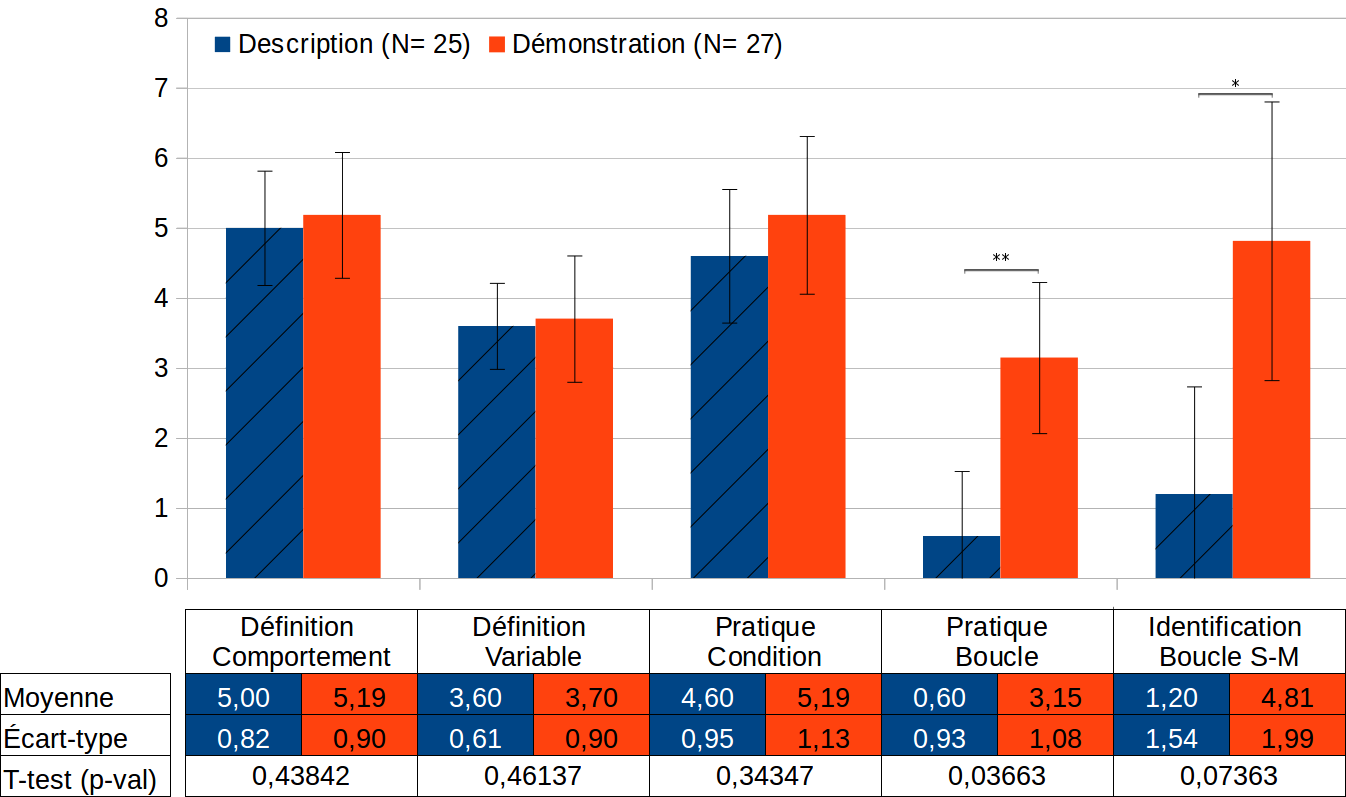
\includegraphics[width=0.9\linewidth]{Figures/Desprez-result_poule-quiz.png}\label{fig:result_poule-quiz}
                \caption{Résultats quiz: \cro{Décrire ou manipuler}}
            \end{figure}\par%
            Sur les cinq questions que comportait ce \sht{QCM}~\citeA{pdf:qcm_poule} seules les deux questions portant sur les boucles ont obtenu des résultats significativement moins bons en condition \sht{GDesc}.
            \begin{enumerate}\myItemStyle
                \item définition; \gui{Qu’appelle-t-on le comportement d’un robot?}
                \item définition; \gui{Qu’est ce qu’une variable?}
                \item illustration; \gui{\sht{snap} vous demande, si tous les moteurs doivent être mis en compliant}
                \item illustration; \gui{Que produisent ces instructions?}
                \item identification; \gui{Parmi ces 10 exemples, où y a t-il une ou plusieurs boucles sensori-motrices}
            \end{enumerate}{}
        \paragraph{Conclusion}
            Nous constatons donc que sur un temps court (sessions d'activités de moins de deux heures) la manipulation directe de la notion à intégrer, ici, la \bg{BSM} est plus favorable. En effet, cette configuration a permis aux élèves non seulement d'améliorer leurs performances au quiz final, mais aussi d'avoir la perception d'avoir fourni moins d'efforts~\citeS{Exp:poule}. Cependant, cette impression de \cro{moindre effort} peut être en décalage. En effet, l'objectif affiché est de réaliser le défi et de produire le comportement \cro{poule} or pour le \sht{GDemo}, cette production est déjà réalisée, pouvant ainsi donner l'illusion de la réussite. Mais, l'objectif pédagogique se trouve ailleurs: le but de cette activité de découverte est de permettre à l'élève d'appréhender et d'identifier une \sht{BSM}. Ainsi, cela a plusieurs avantages: le défi induit par la scénarisation permet d'engager les élèves ou, au moins, de les intriguer. Une fois dans l'activité, fournir une solution tangible permettant d'expérimenter le résultat attendu (ici, le comportement \cro{poule}) offre le double avantage de donner une impression de réussite aux élèves sur leurs objectifs directs (réussite au défi) et d'améliorer \tiret{du moins à court terme} leur compréhension du sujet abordé (ici, la \sht{BSM}. 
    %Reel_virtuel    
    \subsection{\textit{Exp}: \cro{Robot virtuel ou réel, danse avec un robot}}\label{Exp:Reel_virtuel}
        \myPhantom{paragraph}{Introduction}
            Au vu de la difficulté pour certains établissements scolaires de s'équiper en matériel robotique~\citeS{sec:materiel}, nous avons cherché à montrer dans cette expérimentation dans quelle mesure l'utilisation d'une version simulée en tant que substitut à un robot réel \tiret{perdant ainsi les avantages inhérents aux objets tangibles} pouvait avoir un intérêt suffisant. Pour aller plus loin, dans quelle mesure l'aspect tangible est prédominant pour l'apprentissage de la robotique? auquel cas, des ressources comme des \cro{activités débranchées\footnote{(activité en informatique, robotique, numérique, \etc, ne nécessitant pas de matériel informatique, typiquement un ordinateur}} pourraient s'avérer plus efficaces qu'une version simulée d'un robot.
        \subsubsection{Étude pilote}\label{Exp:Reel_virtuel-pilote}
            \paragraph{Méthode}
                Sur une unique session de 2 heures, les élèves ($n=30$) étaient répartis en 2 groupes~V et~R, l'un manipulant le visualisateur ($n=16$), l'autre manipulant le robot réel ($n=14$). L'objectif était d'évaluer la différence qui pourrait exister entre la manipulation d'un robot réel et un robot virtuel simulé.\\
                \sbg{VI}: 
                Quatre conditions: \Li robots réel+virtuel (RV), \ii uniquement la version réel (R), \iii uniquement la version virtuelle (V) et \iiii une activité de démonstration (AD) sans manipulation ni programmation du robot.\\
                \sbg{VD}: 
                \begin{itemize}\myItemStyle
                    \item Motivation, mesurée par questionnaires avant et après expérience
                    \item Connaissances acquises, mesurées par questionnaires après expérience
                    \item Satisfaction, mesurée par questionnaires après expérience
                    \item Réussite, mesure du niveau de progression dans l'activité
                \end{itemize}{}
                \subparagraph{Hypothèses}
                    D'un point vue général, nous pouvons émettre l'hypothèse (qui sera uniquement discutée ici) que la motivation sera maximale lorsque l'étudiant peut manipuler les versions réelles et virtuelles du robot; que la motivation lors de l'utilisation seule du robot réel reste supérieure à l'utilisation seule du visualisateur. Les trois précédentes seront supérieures à la simple démonstration passive des activités; ainsi pour la motivation: RV~>~R~>~V~>~AD.
                    De plus, augmenter la motivation \etou la satisfaction à utiliser un support pédagogique favorise l'acquisition des concepts véhiculés dans ce support; ainsi, nous pouvons supposer que pour la connaissance et la réussite: RV~>~R~>~V~>~AD, si pour la motivation: RV~>~R~>~V~>~AD. 
                    Enfin, nous pouvons émettre comme dernière hypothèse que ces relations seront exacerbées lorsque la satisfaction est positive.
                    Afin d'évaluer au mieux ces hypothèses, il a été décidé de diviser celles-ci en plusieurs sous groupes afin d'effectuer des études pilotes pour étalonner nos activités et nos questionnaires.
                    L'hypothèse intermédiaire (qui sera traitée ici) est que la motivation est supérieure avec le robot réel seul comparé au virtuel seul; ainsi, pour les quatre \sht{VD}:~R~>~V.
                \subparagraph{L'activité}
                    Elle est divisée en deux grandes parties, prise en main (\sht{snap} et robot) et un défi, cette activité propose un déroulement \cro{cadré}: présentation d'une notion/manipulation, exemple, mise en pratique, présentation d'une deuxième, \etc. Cette progression guidée est réalisée par l'élève grâce à un document papier qui lui est fourni~\citeA{pdf:act_dance} et dure entre 30 et 45min. Ensuite un défi est proposé: trouver les 6 paramètres moteurs (position en degrés) afin que le robot atteigne la position donnée dans une photo illustrative; le but étant de trouver un maximum de positions différentes (16 au total) en environ 1~heure.
                \subparagraph{Les questionnaires}
                    Ceux ici utilisés sont des compositions de différents questionnaires existants nous permettant une posture exploratoire quant aux résultats de cette étude pilote. Ainsi, un questionnaire évaluant leur motivation fut effectué avant~\citeA{pdf:qcm-pre_dance} et après l'activité par chaque élève. Des questions additionnelles ont été ajoutées aux questionnaires pré et post activité afin d'identifier chez les élèves leur profil, leur satisfaction et leurs connaissances acquises~\citeA{pdf:qcm-post_dance}. Plusieurs questions relatives aux différents concepts qui englobent la motivation ont donc été posées. Dix-huit éléments étaient communs au questionnaire pré et post-activité. Réparties en différentes catégories, elles évaluent: la motivation intrinsèque (4\sht{ques}) et extrinsèque (4\sht{ques}); l'autodétermination et l'auto-efficacité (6\sht{ques}); les facteurs environnementaux (4\sht{ques}). Ces 18 affirmations (9 positives, 9 négatives) étaient à évaluer suivant une échelle le Likert. Ce questionnaire a été construit suivant différents éléments de la littérature notamment le \sht{SUS} et les résultats de Kaloti-Halla~\citeB{kaloti2015students}.
                    En accord avec Harter~\citeB{harter1981new} cinq affirmations à compléter ont été ajoutées au questionnaire pré-activité pour tenter d'établir des profils d'apprenants. À chaque affirmation trois réponses étaient possibles et rapportaient de 0 à 2 points, déterminant ainsi un score sur~10. Trois profils ont été définis A~(>6), B et C~(<=3).
                    Cinq questions ont été ajoutées au questionnaire post-activité pour évaluer l'acquisition des connaissances. Toutes reliées entre elles, leurs réponses étaient explicitement présentes dans la documentation. Cependant le fait de ne pas évaluer en amont les connaissances induit des restrictions d'interprétation.
                    Toujours dans le questionnaire post-activité, 4 affirmations concernant la satisfaction ont été insérées: \Li\gui{J’ai eu l’impression d’apprendre des choses avec cette activité}; \ii\gui{J’ai trouvé la documentation confuse et incompréhensible}; \iii\gui{Lorsque les choses étaient difficiles, j’ai réussi quand même}; \iiii\gui{Je n’ai pas apprécié cette activité}, également à évaluer selon une échelle de Likert.
            \paragraph{Les résultats}
                Cette expérience pilote a montré qu'une différence existe bien ($p=0.0145$), majoritairement en faveur de l'utilisation du robot réel: La motivation, la satisfaction et la réussite ont été d'un meilleur niveau en condition~R qu'en condition~V, mais aucune différence n'a été observée dans l'acquisition des connaissances. Notons également, que les conditions~R et~V avaient une motivation initiale identique et qu'elle a évolué différemment, notamment avec: une augmentation pour la condition~R dans la catégorie motivation intrinsèque et une diminution pour la condition~V dans la catégorie auto-détermination. Ces résultats traduisent l'effet attendu selon lequel manipuler un objet tangible afin de réaliser son activité, ses essais, est plus efficace, ainsi le niveau de motivation reste stable entre avant et après l'activité, sauf dans la condition~V. Cela peut se traduire également par le fait que les élèves ne se motivent pas pour faire des activités de robotique sans robot tangible. Nous pouvons également supposer que les élèves idéalisent la robotique, ainsi garder le niveau de motivation stable après l'utilisation d'un vrai robot (avec sa complexité et ses contraintes) peut être vu comme une réussite en soi. \par%
                Qualitativement, nous pouvons constater qu'à l'arrivée des sujets aucune différence ne semblait être relevée. Suivant s'ils passaient la condition robot réel~(R) ou virtuel~(V) ils ont été répartis en 2 groupes pour passer le questionnaire. Très rapidement après le début de l'activité une distinction s'est réalisée au niveau de l'ambiance générale de la classe: la condition~R était largement plus \cro{bruyante} que la condition~V extrêmement concentrée sur l'ordinateur. Les dialogues dans le groupe et entre les groupes ont semblé beaucoup plus fréquents dans la condition~R. De plus, la possibilité de voir et d'entendre les mouvements des autres robots dans la condition~R a semblé, parfois dynamiser la classe en stimulant l'esprit de compétition (\cro{S'il y arrive alors je dois pouvoir y arriver}), et parfois distraire les élèves de leur propre réalisation. À la fin de l'activité plusieurs élèves de la condition~R étaient \cro{déçus} qu'elle soit finie, ce type de réaction n'a pas été observée dans la condition~V. Enfin tous les groupes de la condition~R semblent avoir participé activement pendant les 2h d'activité, quand certains groupes de la condition~V ne totalisent que 5 instructions, ou moins, envoyées au robot. Comptabiliser systématiquement le nombre d'instructions envoyées au robot pourrait fournir des informations pertinentes sur l'engagement de l'élève et plus généralement, des mesures quantitatives directement issues des logs permettraient également de lever certaines ambiguïtés.\par%
                Les nombreuses interprétations contradictoires mises en avant ici ne permettent pas de dégager une cohérence globale entre tous ces résultats. Cependant cette conclusion était attendue car l'objectif de ces études pilotes est avant tout de calibrer un questionnaire plus attentif aux phénomènes que nous cherchons à mettre en évidence avec des activités pertinentes sur un support éprouvé et non d'établir des conclusions générales. Notamment, car d'autres facteurs ont dû être omis, comme les connaissances antérieures que possèdent les sujets ou encore la durabilité des connaissances acquises. De plus, plusieurs biais ont pu être relevés dans l'évaluation de la motivation et dans la comparaison d'activités ayant le même protocole: principalement nous observons des différences significatives dans les évaluations pré-activité entre les conditions (réel~/~virtuel), cela peut-être dû au lieu et l'horaire de passation, à l'expérimentateur(s) présentant l'activité, \etc. Enfin L'utilisation de différents supports (vidéos~/~textes) semble également induire des distinctions qui, dues à la variabilité du niveau de motivation initiale, sont difficiles à interpréter. 
            \paragraph{Conclusion},
                Cette expérience pilote ne permet donc pas d'anticiper les résultats d'une étude plus large, notamment sur la corrélation entre niveau de motivation et satisfaction et sur un niveau de motivation plus élevé en condition~R qu'en condition~AD. Mais des pistes de recherche ont été ouvertes, et un certain nombre de cycles expérimentaux devront être itérés pour essayer de conclure sur ce sujet.
        \subsubsection{Étude contrôlée}\label{Exp:Reel_virtuel-control}
                Suite à cette étude pilote, nous avons souhaité nous focaliser sur l'aspect facilitateur que pouvait revêtir les conditions~R et~V sur l'acquisition de compétences particulières notamment sur les habiletés visuo-spatiales fortement nécessaires dans l'activité Danse~\citeA{pdf:act_dance}. 
                Trois conditions seraient constituées: robot réel~R, virtuel~V et \cro{cube de construction}~C, après une présentation commune \tiret{n'évoquant pas les activités} ces 3 groupes sont séparés. Après le démarrage des activités, une partie de chaque groupe (environ 25\prc[)] compléterait une série de questions basées sur les tests de rotation mentale de Vandenberg~\citeB{vandenberg1978mental}, étalonnées en 1996 pour les 15-19~ans par Albaret~\citeB{Albaret1996test}. Ces questions devront être intégrées directement dans les activités afin de ne pas attirer l'attention des autres élèves. Cette population servira à déterminer notre ligne de base pour ce test par rapport aux différentes conditions de passations (type de classe, horaires, \etc). 
                L'activité pour les conditions~R et~V est basée sur l'activité Danse comme précédemment et constitue ici une phase d'entraînement pour le test final, un test de rotation mentale. Le groupe~C aurait, quant à lui, des instructions n'ayant pas de rapport direct avec la robotique, mais préparant également au test final; il représente notre condition témoin. 
                Ce test de rotation mentale serait complété par le \sht{SUS} et l'\sht{ATT} pour les conditions~R et~V, et par des sous-échelles du \sht{IMI} pour les 3 conditions. Comme pour le test de rotation mentale, une partie de la population effectuerait les passations à différents moments \ie avant toute chose, après l'activité ou après le test final de rotation mentale.
                Cependant, faute de temps, cette expérimentation est encore en préparation et n'a pas été réalisée.
    \subsection{Synthèse}
        Étudier l'acquisition de connaissances nécessite un temps long et plusieurs temps de mesures, or nous n'avons pas été en mesure de mettre un place un tel dispositif dans les délais impartis. Cependant, relever certains éléments ponctuels lors d'autres études permet de mieux interpréter les résultats obtenus, comme pour l'expérience présentée en début de ce sous-chapitre, où nous avons vu que le sentiment d'effort perçu (\ie faible) été associé à une meilleure compréhension du concept et pas uniquement à l'impact du type de démonstration. De plus, dans le cadre d'activités traitant de compétences spécifiques (ici visuo-spatiale), s'assurer que les avantages prédits pour l'utilisation d'objets tangibles sont bien présents et significatifs dès la première mise en place, représente une étape indispensable à l'étude plus approfondie de telles dimensions sur le long terme. 